\section{Week 2: Purity of Thought}

The distinguishing mark of the Hermetic path is that it seeks to make dogmas and teachings “real” in consciousness. As
Tomberg insists, this does not make it “better” than the exoteric teaching, only that it is a path that some are called
to follow.

In this spirit, we can meditate on what \textbf{Christmas} means.

\begin{itemize}
\item The birth in the past of Christ the Redeemer. 
\item The expectation of Christ the Judge at the end of time. 
\item The birth of Christ in the soul eternally, now. 
\end{itemize}

\begin{wrapfigure}{tr}{.3\textwidth}
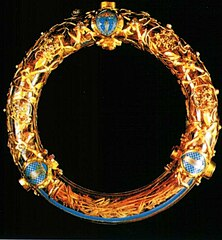
\includegraphics[scale=.5]{x20221202AdventMeditationWeek2-img001.jpg}
\caption{Relic of the crown of thorns}
\end{wrapfigure}
Redemption is the reversal of the effects of the Fall. The Hermetic Tradition calls this process “regeneration” as we
seek to make that real in consciousness. The undoing of the Fall requires the second birth of Christ/Logos in the soul.
That is, the soul, as the passive element, reflects the activity of the Spirit. Disturbances in the soul
— passions, images, desires, thoughts — will distort the reflection of
spirit, just as disturbances on a pond distort its reflection of the surrounding forest.

It is this personal, subjective element that is at the root of such disturbances. Thus, the solution is to become more
objective about oneself. That is to take the standpoint of Christ the Judge. Justice is possible only when the Judge is
totally objective, not influenced by ignorance, opinion, personal preferences, or subjective passions. \textbf{Valentin
Tomberg} writes in this regard:

\begin{quotationx}
The vow of \emph{obedience} is the practice of silencing personal desires, emotions and imagination in the face of
reason and conscience; it is the primacy of the ideal as opposed to the apparent, the nation as opposed to the
personal, humanity as opposed to the nation, and God as opposed to humanity. It is the life of cosmic and human
hierarchical ordering; it is the meaning and justification of the fact that there are Seraphim, Cherubim, Thrones;
Dominions, Virtues, Powers; Principalities, Archangels, Angels; Priests, Knights and Commoners. Obedience is order: it
is international law; it is the state; it is the Church; it is universal peace. True obedience is the very opposite of
tyranny and slavery, since its root is the love which issues from faith and confidence. That which is above serves that
which is below and that which is below obeys that which is above. Obedience is the practical conclusion to that which
one recognises as the existence of something higher than oneself. Whosoever recognises God, obeys. 

\end{quotationx}

Yet that does not address the question of “how” to obey. We cannot obey as long as the subjective element has its grip
on us; these are impure elements that disturb the soul. Tomberg discusses the idea of purity in the context of the five
wounds and three vows. We can summarize these in two stages: purity of thought and purity of will. These correspond to
the head and the heart respectively.

Purity of thought is the “crown of thorns”. The following passages explain that symbol:

\begin{quotationx}
Thus every crown is essentially a crown of thorns. Not only is it heavy, but also it calls for a painful restraint with
regard to the thought and free or arbitrary imagination of the personality.

Here true thought receives confirmation and subsequent illumination; false or irrelevant thought is riveted and reduced
to impotence. The crown of the Emperor signifies the renunciation of freedom of intellectual movement, just as his arms
and legs signify his renunciation of freedom of action and movement. He is deprived of the three so-called “natural”
liberties of the human being — those of opinion, word, and movement.

The “crown of thorns” is borne, in principle, by every person capable of \emph{objective} thought —
the “crown of thorns” being given to the human being since the beginning of human history. 

\end{quotationx}

The lack of concentration allows arbitrary, free, or irrelevant thoughts and images to flourish in our consciousness. We
need to renounce them so they can be replaced by true thoughts; the art of concentration will help in that regard.

\textbf{Nicholas Cabasilas} writes this in his commentary on the beatitude of “purity of heart”.

\begin{quotationx}
To cleanse one's heart and to exercise one's soul for sanctification
— what striving or effort or exertion would effect this more than these thoughts and meditations?
Yet, if one examines this carefully, one would not call it the effect of meditation on Christ, but rather of the
meditation itself.

To be occupied with the noblest of thoughts means to abandon evil thoughts; but this is to be pure in heart. Our life
and our birth are twofold, both spiritual and fleshly. By its desires, the spirit fights against the body and the body
resists the spirit. Since it is impossible for contraries to be at peace and to join together, it is quite evident that
one or other of the desires will by means of memory, gain control over the thoughts and cast the other out. The memory
of the life and birth which are according to the flesh and concentration on such matters produce the most depraved
desires and the uncleanness to which it leads. So likewise, when the soul by constant remembrance holds fast the birth
of the baptismal washing, the divine Food which is appropriate to this birth, and the other things which belong to the
new life, it is likely to lead desires from the earth to heaven itself. 

\end{quotationx}
We can extract these main points:

\begin{itemize}
\item There is our fleshly birth in the body and a second spiritual birth. 
\item There is an inner spiritual battle between lower (personal, subjective) thoughts and higher (spiritual, objective)
thoughts 
\item “Constant remembrance” is necessary. In our terms, this is constant awareness, “concentration without effort” 
\end{itemize}
Hermetically, this movement from fleshly to spiritual thoughts is a mystical evolution. This is the regeneration of the
inner life from the Instincts to fully human life of the Intellect and Intuition.

For more on this, you could start with \textit{Salvation and Evolution}\footnote{}.

As for the idea of regeneration, it is necessary to understand what the Fall entailed. Given
Tomberg's high opinion of Jacob Boehme, this summary of Boehme's teaching may
be helpful, especially the sections on the Fall of Lucifer and Adam's Fall: \textit{Christian Gnosis: Jacob Boehme}\footnote{}.

\flright{\itshape Posted on 2022-12-02 by Cologero}
